\chapter{基于视角迭代自注意力控制的数字人外观生成}
\section{本章引言}
上一章从动作生成角度解决了三维数字人的舞蹈表现力问题，而三维数字人舞蹈内容生成的另一项核心挑战在于数字人外观的个性化编辑与生成。外观不仅决定了数字人的视觉辨识度与角色身份认同，同时也是影响整体舞蹈表现力与真实感的重要因素。在虚拟偶像演出、沉浸式社交及数字娱乐等应用场景中，用户往往需要根据不同的演出主题、角色设定或个人审美对数字人的外观进行快速定制——例如更换服饰风格、调整发型配饰、甚至迁移特定艺术风格等。因此，如何在保持多视角一致性的前提下，高效地实现三维数字人外观的个性化编辑，是构建高表现力数字人舞蹈内容的关键环节。

围绕这一问题，现有个性化外观编辑方法主要可归纳为两类范式：基于模型训练的方法与基于注意力机制的方法。基于模型训练的方法~\cite{brooks2022instructpix2pix,chen2023anydoor,yang2022paint}通常依赖构建数据集并对整个模型进行微调，因而带来较大的时间与算力开销。为避免昂贵的训练成本，近年来研究者提出了基于注意力机制的方法~\cite{hertz2022prompt,mokady2022null,cao2023masactrl,parmar2023zero}，其核心思想是在扩散模型的U-Net中直接操控注意力机制从而控制模型生成的内容。例如，Prompt-to-Prompt~\cite{hertz2022prompt}通过仅编辑文本提示词并在扩散过程中注入交叉注意力图实现图像编辑；MasaCtrl~\cite{cao2023masactrl}则利用互自注意力机制，从源图像中查询相关的局部内容与纹理，实现非刚性且一致的图像编辑。面向视频与三维场景等其他视觉模态的编辑方法，大多建立在上述图像编辑技术之上~\cite{instructnerf2023,ceylan2023pix2video}。然而，将现有二维图像编辑方法应用于三维数字人外观编辑时，在效率、稳定性与跨视角适用性方面仍面临若干关键挑战：
\begin{enumerate}
\item \textbf{外观身份保持受限。} 仅依赖文本描述进行控制时，文本本身存在固有的歧义性与表达不精确性，往往导致生成结果在外观细节与身份特征上偏离用户期望~\cite{cao2023masactrl}。对于三维数字人而言，外观身份的不一致将直接破坏角色的视觉辨识度，影响观众对数字人角色的认知连贯性。此外，在多数文生图扩散模型中，即便对提示词进行微小调整，也可能引发显著的外观变化~\cite{hertz2022prompt}，从而难以稳定地保持目标主体的外观身份一致性。

\item \textbf{训练代价高且推理效率受限。} 现有基于反演或微调的方法通常依赖冗长的DDIM反演或额外的模型参数更新过程，这不仅显著增加了计算开销，还可能导致潜空间表示逐步偏离原始轨迹，从而产生不理想的重建与编辑结果~\cite{mokady2022null}。这类方法在实际应用中难以满足用户快速进行数字人外观定制的需求，尤其在需要频繁更换角色造型的虚拟演出场景中效率瓶颈更为突出。

\item \textbf{多视角一致性不足，难以支撑三维数字人应用。} 现有方法大多针对单视角或静态图像设计，难以在跨视角生成过程中保持外观与结构的一致性。然而，三维数字人的外观编辑天然要求在多个视角下保持统一的视觉效果。当直接将现有二维编辑方法应用于三维场景（如基于3DGS的数字人模型）时，不同视角间的编辑不一致会破坏几何一致性，导致三维重建产生严重伪影，从而无法满足高质量数字人渲染的需求。
\end{enumerate}

% \begin{figure}[t]
%   \centering
%   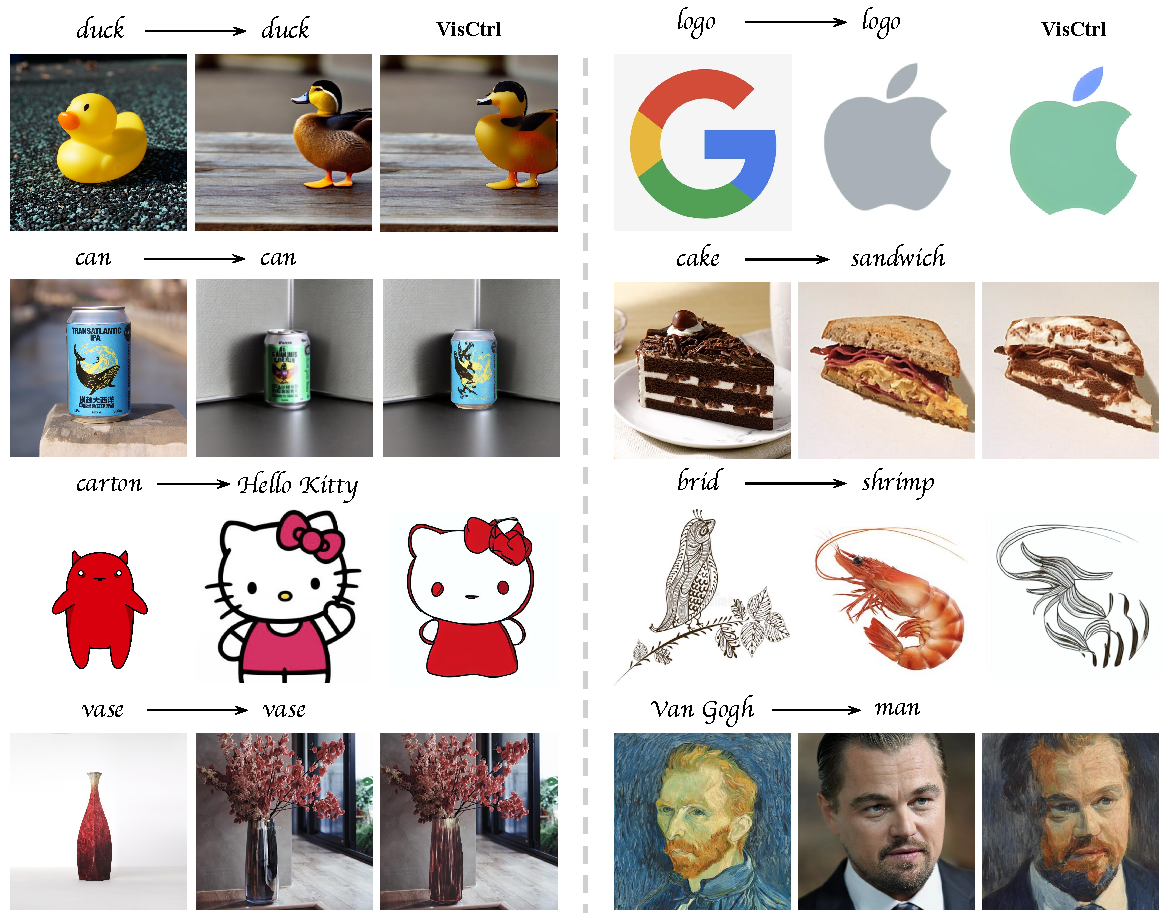
\includegraphics[width=1.000\textwidth]{./figures/VisCtrl/show_res.pdf}
%   % \vspace{-5mm}
%   \caption{VisCtrl方法的编辑效果示例。该方法能够在保持源图像布局结构的同时，将参考图像中的个性化外观特征注入目标图像，为三维数字人外观定制提供二维层面的基础编辑能力。}
%   % \vspace{-5mm}
%   \label{fig:visctrl_show_res}
% \end{figure}

为应对上述挑战，本章提出视角迭代自注意力控制（View Iterative Self-Attention Control，VisCtrl），一种简洁且有效的个性化视觉编辑框架，利用自注意力机制将参考图像中的个性化主体特征注入到目标图像中。具体而言，本章首先通过DDIM反演~\cite{song2021ddim}分别获得参考图像与目标图像对应的初始噪声；随后在去噪重建过程中，采用迭代式自注意力机制，将用户指定主体的特征逐步注入目标图像，同时利用交叉注意力机制维持目标图像的整体结构不变。进一步地，本章提出特征渐进采样（Feature Gradually Sampling，FGS）策略以支持三维数字人外观编辑：该策略通过对参考图像的潜变量特征进行随机采样，在多视角之间实现一致的外观特征注入，从而将二维编辑能力自然拓展至三维场景。
%值得注意的是，在无需重训练、仅使用单张参考图像的条件下，本章所提方法仍可通过较少的去噪步数获得如图~\ref{fig:visctrl_show_res}所示的优异结果。

本章的技术路线遵循先从二维基础验证再通过多视角一致性扩展到三维数字人外观编辑的递进逻辑：首先在二维图像层面验证所提出的无训练个性化特征注入能力，随后通过特征渐进采样策略将其扩展至多视角一致的三维数字人外观编辑场景，最终服务于三维数字人的高效外观定制需求。通过大量实验验证了所提方法的有效性，本章的主要贡献总结如下：

\begin{itemize}
\item 提出了一种无需训练的个性化视觉编辑框架，仅依赖单张参考图像即可完成数字人外观定制，在显著降低训练代价的同时实现高效推理，为三维数字人的快速外观迭代提供了良好的可扩展性。

\item 设计了迭代式自注意力控制机制，在生成过程中联合参考图像及其对应的文本条件，对外观特征进行逐步注入与约束，从而有效保持数字人外观身份的一致性，并避免对整体结构与布局的破坏。

\item 提出了面向三维数字人的特征渐进采样策略，通过在多次迭代中平滑融合来自不同视角的外观信息，显著提升生成结果在跨视角场景下的一致性，从而将所提框架自然拓展至基于3DGS的三维数字人外观编辑任务。

\end{itemize}

\section{视角迭代自注意力控制}
\subsection{扩散模型反演}
潜空间扩散模型~\cite{Rombach_2022_CVPR_stablediffusion}主要由两部分组成：自编码器与潜空间扩散模型。自编码器中的编码器$\encoder$将输入图像$\inputimage$映射为潜变量代码$z_0=\encoder(\inputimage)$，解码器则将潜变量代码还原为图像，满足$\decoder(\encoder(\inputimage)) \approx \inputimage$。令$\textembedding=\conditioner(\textprompt)$表示条件机制，将文本条件$\textprompt$映射为潜空间扩散模型的条件向量，则其训练目标可写为：
\begin{equation}
L_{LDM} := \mathbb{E}_{z_0 \sim \encoder(\inputimage), \textprompt, \epsilon \sim \mathcal{N}(0, 1), t \sim \text{U}(1,T) }\Big[ \Vert \epsilon - \model(z_{t},t, \textembedding) \Vert_{2}^{2}\Big], \, 
\label{eq:ldm_loss}
\end{equation}
其中去噪网络$\model$通常为条件U-Net~\cite{ronneberger2015unet}，用于在时间步$t$预测所加的高斯噪声$\epsilon$。文本生成图像扩散模型~\cite{saharia2022photorealistic, ramesh2022hierarchical, rombach2022high,nichol2021glide}通常采用式~\ref{eq:ldm_loss}进行训练，即在给定文本提示$\textprompt$的条件下，使$\model$学习估计噪声。


DDIM反演~\cite{song2021ddim}的目标是在给定文本条件$\textprompt$的情况下，寻找一个初始噪声$z_T$，使其能够重建输入潜变量代码$z_0$。由于本章的目标是结合参考图像实现对给定图像的精确重建，因此采用确定性DDIM采样~\cite{song2021ddim}：
\begin{equation}
z_{t+1} = \sqrt{\bar{\alpha}*{t+1}}f*\theta(z_t,t,\textembedding) + \sqrt{1-\bar{\alpha}*{t+1}} \model(z_t,t,\textembedding)
\label{eq:ddim}
\end{equation}
其中$\bar{\alpha}*{t+1}$为DDIM~\cite{song2021ddim}中定义的噪声缩放系数，$f_\theta(z_t,t,\textembedding)$用于预测最终去噪后的潜变量代码$z_0$，其形式为：
\begin{equation}
f_\theta(z_t,t,\textembedding) = \Big[z_t - \sqrt{1-\bar{\alpha}_t} \model(z_t,t,\textembedding) \Big] / {\sqrt{\bar{\alpha}_t}}.
\end{equation}
潜空间扩散模型中的注意力机制由U-Net中一系列基础模块构成，每个基础模块通常包含残差块~\cite{he2016deep}、自注意力模块以及交叉注意力模块~\cite{vaswani2017attention}。注意力机制可形式化为：
\begin{equation}
\label{eq:attention}
\text{Attention}\mathcal(Q_t, K, V)= softmax(\frac{Q_{t}K^T}{\sqrt{d}})V,
\end{equation}
其中$d$表示潜变量特征维度；$Q$表示由空间特征投影得到的查询特征；$K$与$V$分别表示键与值特征，它们在自注意力层中由空间特征投影得到，而在交叉注意力层中则由文本嵌入投影得到。对应的注意力图为
$
\mathcal{A}_t=softmax(Q_t \cdot K^T / \sqrt{d}),
$
即式~\ref{eq:attention}中的第一项。

\begin{figure}[t]
  \centering
    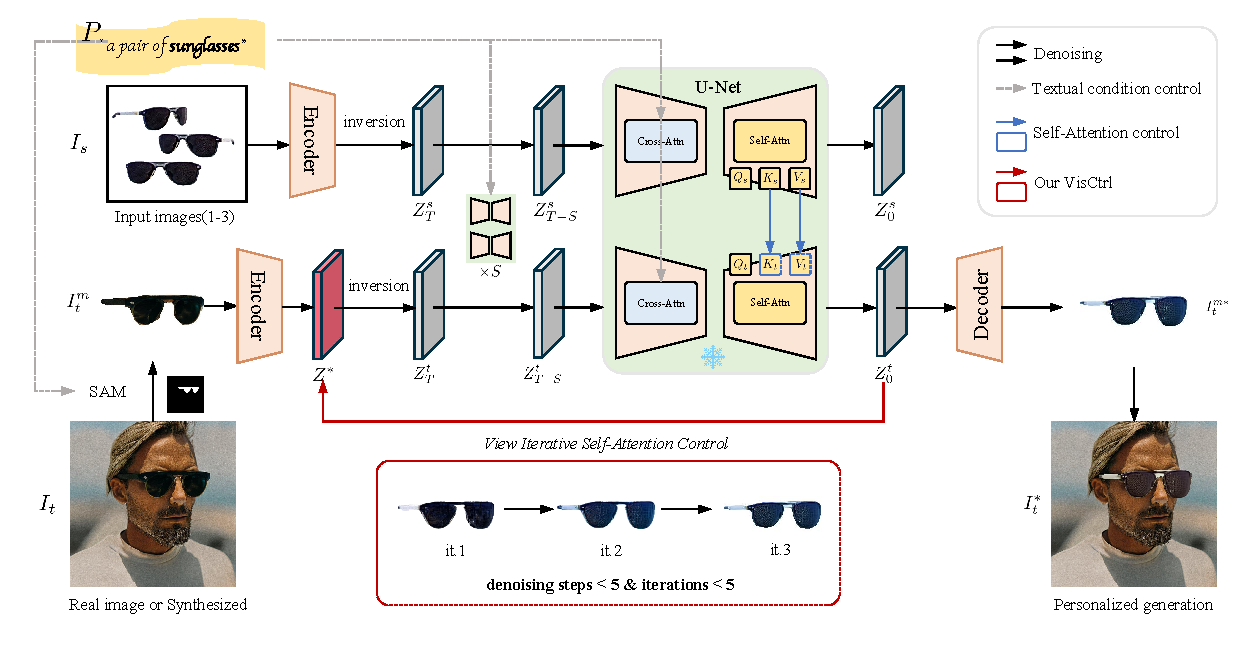
\includegraphics[width=1.000\textwidth]{./figures/VisCtrl/framework.pdf}
  % \vspace{-1mm}
  \caption{VisCtrl视觉生成与编辑算法框架}
  % \vspace{-3mm}
  \label{fig:visctrl_pipeline}
\end{figure}


\subsection{算法架构}
\label{sec:visctrl}
如图~\ref{fig:visctrl_pipeline}所示，VisCtrl架构包含参考图像分支（上）与目标图像分支（下）。给定一张或多张用于表征新概念的参考图像，首先将其通过编码器映射到潜空间，随后添加噪声。两条分支均执行反演与去噪过程，但二者的去噪流程有所不同。具体而言，参考图像分支通过自注意力提供个性化的主体特征；随后，在目标图像分支中，按照如下方式组装自注意力的输入：（1）保持当前的查询特征$Q_t$不变；（2）从参考图像分支的自注意力层中获取$K_s$与$V_s$特征；（3）持续执行上述去噪过程以获得$Z_0^t$；（4）将$Z_0^t$用作$Z^*$的替代值，并在其后进行一次反演过程，然后重复步骤（1）至（3）共计$N$次迭代，从而将参考图像的特征逐步注入到目标图像中。最后，将$Z_0^t$通过解码器还原到像素空间，得到编辑后的目标图像。$Z^*$初始化为$\encoder(I_t)$，在迭代过程中按照如下公式更新：
\begin{equation}
\label{eq:z_star}
Z^**{(n+1)} = Z^t*{0(n)}, \quad 1 < n < N
\end{equation}
其中，$n$表示迭代次数，$N$为总迭代次数。值得注意的是，仅在5次迭代内即可获得显著提升。每次迭代包含一次反演过程与一次去噪过程，且两者的步数均不超过5步。更进一步地，通过为编辑选择合适的去噪起始步$S$与层索引$L$，可以控制参考图像在外观与结构层面向目标图像注入的程度。
%具体效果如图~\ref{fig:visctrl_diff_step}所示，其中右上行展示了在不同去噪步数设置下的生成结果，右下行则在$T=10$的条件下给出了采用不同注入步时的生成结果。
VisCtrl算法的伪代码如算法~\ref{alg:visctrl}所示：
% \begin{wrapfigure}{r}{1.0\textwidth}
% \vspace{-5mm}
% \hspace{2mm}
% {
\begin{algorithm}[H]
\SetAlgoLined
\textbf{Input:}The reference images $\{I_s\}_1^N$ and corresponding prompt $\textprompt_s$, a target image$I_t$ and corresponding prompt $\textprompt_t$.\\

\textbf{Output:} Edited latent map $z^t_0$. \\
$\{z^s_T\}_1^N\leftarrow \text{DDIMInversion}(\encoder(\{I_s\}_1^N),\textprompt_s)$;\\
$z^*=\encoder(I_t)$;\\
$z^t_T\leftarrow \text{DDIMInversion}(z^*,\textprompt_t)$;\\
\For{$n=N,N-1,\ldots,1$}{
$z^t_T \leftarrow \alpha * \text{DDIMInversion}(z^*,\textprompt_t) + (1-\alpha)*z^t_T$;\\
$z^s_T=\text{DataSampler}(\{z^s_T\}_1^N)$;\\
 \For{$t=T,T-1,\ldots,1$}{
    $\epsilon_s, \{Q_s, K_s, V_s\}\leftarrow \epsilon_\theta(z^s_t, P_s, t)$;  \\ 
    $z^s_{t-1} \leftarrow \text{DDIMSampler}(z^{s}_{t}, \epsilon_s)$;\\
    $\{Q_t, K_t, V_t\} \leftarrow \epsilon_\theta(z_t,P,t)$;\\
    $\{Q_t^*, K_t^*, V_t^*\} \hspace{-1mm}\leftarrow \text{Edit}(\{Q_t,K_t,V_t\}, \{Q_s, K_s, V_s\})$;\\
    $\epsilon_t = \epsilon_\theta(z_t, P, t; \{Q_t^*, K_t^*, V_t^*\})$;\\
    $z^t_{t-1} \leftarrow \text{DDIMSampler}(z_t^t, \epsilon_t)$;\\
 }
 $z^* =z^t_0$;\\
}
 \textbf{Return} $z^t_0$ \\
 \caption{View Iterative Self-Attention Control}
\label{alg:visctrl}
\end{algorithm}
% }
% \end{wrapfigure}

其中，算法~\ref{alg:visctrl}中的$\text{注意力编辑}(\{Q_t,K_t,V_t\}, \{Q_s, K_s, V_s\})$可形式化为：当去噪时间步$t$大于阈值$S$且网络层级$l$大于阈值$L$时，将目标分支自注意力层中的键和值替换为参考分支对应的$K_s$和$V_s$，仅保留目标分支的查询$Q_t$；否则保持目标分支原始的查询、键、值不变。$S$与$L$分别表示开始注入的时间步与层索引。

% 其中，算法~\ref{alg:visctrl}中的编辑函数Edit可形式化为：
% \begin{equation}
%     \label{eq:visctrl_edit}
%     \text{Edit} := \left \{
%     \begin{aligned}
%         & \{Q_t, K_s, V_s\},\quad \text{if}\quad t > S \quad \text{and} \quad l > L, \\
%         & \{Q_t, K_t, V_t\},\quad \text{otherwise},
%     \end{aligned}
%     \right.
% \end{equation}


% \begin{figure}[!th]
%   \centering
%     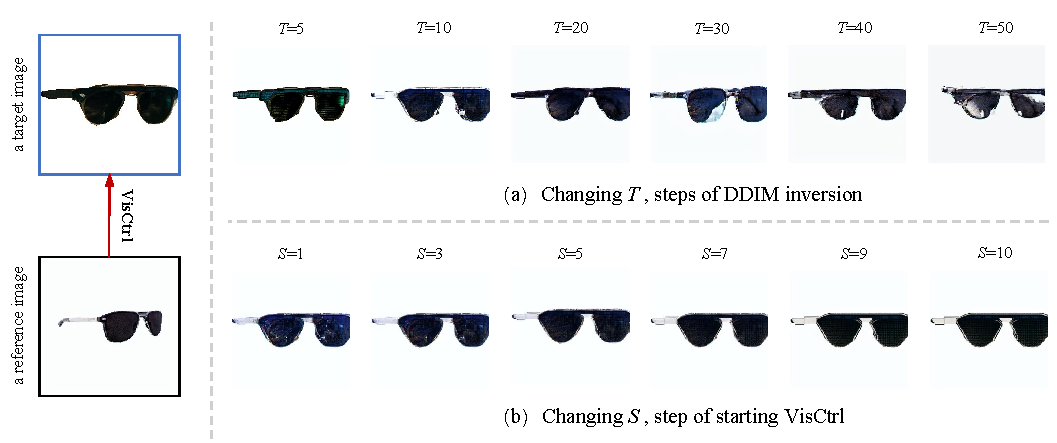
\includegraphics[width=1.000\textwidth]{./figures/VisCtrl/diff_step.pdf}
%   % \vspace{-1mm}
%   \caption{操控不同去噪步数和网络层索引的编辑结果对比}
%   % \vspace{-3mm}
%   \label{fig:visctrl_diff_step}
% \end{figure}


\section{面向三维数字人的特征渐进采样策略}
将VisCtrl方法从二维图像编辑拓展至三维数字人外观编辑时，需要对基于3DGS等三维表示的数字人模型进行多视角一致的外观修改。然而，三维数字人的训练数据通常包含从多个视角拍摄的图像，直接对这些多视角图像逐一进行独立编辑将面临两个关键挑战。\textbf{（1）单参考图像的信息量有限：}在三维数字人的多视角数据中，不同视角之间的外观变化显著。仅依赖单张参考图像往往因可用信息不足而导致生成结果模糊，使目标图像在迭代过程中逐渐丢失其原始结构。一旦结构被破坏便难以恢复，因为缺失的结构信息已不再存在于目标图像的查询特征中。\textbf{（2）多视角编辑的一致性：}三维数字人的外观编辑对跨视角一致性有严格要求——不同视角间的编辑差异会直接破坏三维重建所需的几何一致性，导致3DGS等三维模型在训练时无法稳定收敛，最终在渲染结果中产生严重伪影。因此，必须确保来自多张参考图像的信息注入保持一致。

\begin{figure}[t]
  \centering
    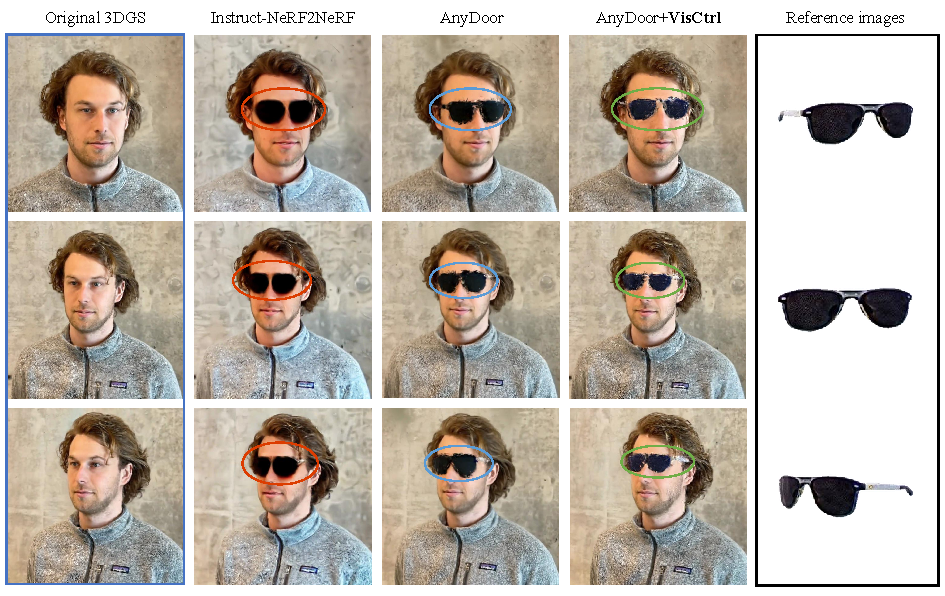
\includegraphics[width=1.000\textwidth]{./figures/VisCtrl/3d_editing_baseline.pdf}
  % \vspace{-1mm}
  \caption{不同方法在三维数字人外观编辑任务上的结果对比}
  % \vspace{-3mm}
  \label{fig:visctrl_3d_baseline}
\end{figure}

因此，本章提出面向三维数字人多视角编辑的特征渐进采样（FGS）策略。该策略通过对参考图像中的数据进行随机采样，使目标图像能够感知尽可能多的有效信息，从而在编辑三维数字人各视角图像时获得更完整的外观特征。此外，为缓解迭代过程中的遗忘问题，对$z$采用加权更新。$Z^t_{T(n+1)}$的更新公式如下：
\begin{equation}
\label{eq:z_t}
Z^t_{T(n+1)} = \alpha * \mathcal{F}(Z^**{(n)}, \textprompt_t) + (1-\alpha)*Z^t*{T(n+1)}, \quad 1 < n < N
\end{equation}
其中，$n$表示迭代次数，$\mathcal{F}$表示目标分支的DDIM反演过程，即在文本条件$\textprompt_t$下利用$Z^*_{(n)}$获得初始噪声。参数$\alpha$为采样系数，用于控制特征注入的程度；较小的$\alpha$会带来更渐进的特征变化。

\section{实验设计与结果分析}
\subsection{实验配置}
本章在多种实验场景中基于Stable Diffusion v1.5~\cite{Rombach_2022_CVPR_stablediffusion}验证了所提方法的有效性。为体现本章方法从二维基础验证到三维数字人外观编辑的递进逻辑，实验依次涵盖二维图像编辑（基础能力验证）、视频逐帧编辑（时序一致性验证）与三维场景编辑（核心应用验证）三个层面。实验中采用的分割模型为LangSAM，该算法构建于SAM~\cite{kirillov2023segany}与GroundingDINO~\cite{liu2023grounding}检测模型之上。所有实验均在单张NVIDIA V100 GPU上完成。

\textbf{二维图像编辑的配置。} 为验证VisCtrl在外观特征注入方面的基础能力，首先在二维图像编辑场景下与现有方法进行对比。AnyDoor~\cite{chen2023anydoor}与Paint-by-Example~\cite{yang2022paint}属于基于模型的方法，需要在大规模数据集上进行充分微调。实验中使用了其各自论文中描述的默认模型与参数设置：给定一张源图像及其掩码，参考图像会被插入到对应的掩码区域中。Photoswap~\cite{gu2023photoswap}与VisCtrl属于基于注意力的方法，通过操控U-Net中的注意力机制实现图像编辑。然而，与Photoswap不同的是，Photoswap需要通过Dreambooth~\cite{ruiz2022dreambooth}从参考图像中学习新概念，而VisCtrl不需要任何额外的训练或学习过程。为保证公平性，由于VisCtrl仅使用一张参考图像，Photoswap中同样仅使用单张图像来学习新概念，其Dreambooth训练步数设置为1000，其余参数保持默认。对于本章方法，加噪与去噪步数均设置为$T=5$，无分类器引导系数设置为$\omega=6$，迭代次数设置为$N=5$。首先使用DDIM反演~\cite{song2021ddim}将参考图像与目标图像均转换为初始噪声，然后进行去噪并迭代直至收敛。增大步数能够注入并生成更多细节，但不宜设置过大，以避免引入DDIM反演带来的显著偏置。通常而言，在初始迭代中可以设置较高的步数以捕获更多细节，而在后续迭代中去噪步数保持为5。该方法具有很高的效率，一般在三次迭代内即可收敛并获得令人满意的结果。需要注意的是，在二维图像实验中仅使用了一张参考图像。

\textbf{视频编辑的配置。} 视频编辑实验用于验证VisCtrl在时序场景下维持一致性的能力，这一能力是实现三维多视角一致编辑的重要过渡。在视频编辑任务中，将所提方法应用于逐帧编辑的设置，即对视频的每一帧分别进行编辑。由于支持参考图像输入的视频编辑方法较少，本章将所提方法与其他由文本驱动、无需微调的视频编辑模型进行比较，例如Pix2Video，以代表常见的视频编辑方法。对于本章方法，每一帧都提供一张参考图像进行编辑，以期实现整体一致的编辑效果。对于Pix2Video，获取参考图像的文本描述并将其作为文本输入来实现视频编辑。实验中Pix2Video的无分类器引导系数设置为$\omega=3.5$，DDIM步数设置为$T=50$。由于Pix2Video不支持参考图像输入，本章不对编辑结果与参考图像之间的相似性进行过多讨论，而是更关注编辑后视频的时序一致性以及背景的保留程度。

\textbf{三维数字人外观编辑的配置。}
三维数字人外观编辑是本章方法的核心应用场景。在基于文本的三维场景编辑实验中，选择Instruct-NeRF2NeRF作为基线方法之一~\citep{instructnerf2023}。首先使用NeRFStudio~\citep{tancik2023nerfstudio}中的\emph{splatfacto}方法~\citep{igs2gs}对3DGS~\cite{kerbl3Dgaussians}进行预训练，在一张NVIDIA Tesla V100上以10分钟训练30,000步。随后，以"give him a pair of sunglasses"作为Instruct-NeRF2NeRF的文本条件，对三维场景及其对应数据集进行迭代式编辑。由于目前个性化三维场景编辑方法较少，本章进一步采用二维编辑方法（如AnyDoor~\citep{chen2023anydoor}）作为另一类三维场景编辑的基线：先使用这些二维方法对三维场景数据集中的多视角图像进行编辑，然后再训练3DGS模型以获得编辑后的三维场景。在使用AnyDoor对每张图像进行编辑时，保持模型默认参数不变，并开启形状控制的配置项。该实验流程直接模拟了三维数字人外观定制的实际应用场景：通过对多视角训练图像进行一致性编辑，实现对三维数字人模型外观的修改。


\subsection{评估指标与量化结果分析}
\subsubsection{评估指标}
在定量评估中，从三个维度进行衡量：（1）从参考图像中注入特征的充分性；（2）编辑后图像对源图像结构的保留程度；（3）图像间背景区域的一致性。具体而言，使用CLIP-I~\cite{ruiz2023dreambooth}衡量参考图像与生成图像在主体层面的保真度，该指标通过计算生成图像与真实图像在CLIP~\cite{radford2021learning}嵌入空间中的平均两两余弦相似度获得。此外，计算背景LPIPS误差（BG LPIPS）用于量化编辑后背景区域的保留情况：该指标计算源图像与编辑后图像在背景区域上的LPIPS距离，其中背景区域通过SAM目标检测器~\cite{kirillov2023segany}进行识别，得分越低表示背景保留效果越好。最后，采用结构相似性指标（SSIM）评估源图像与生成图像之间的相似度，以确保生成结果能够保持源图像的整体结构。在视频编辑与三维场景操控任务中，同样使用CLIP-I与LPIPS指标进行评估。此外还使用CLIP方向相似度~\cite{gal2021stylegannada}，用于量化文本修改方向与对应图像变化方向之间的一致性程度。

\subsubsection{量化结果分析}

VisCtrl能够便捷地迁移并适配到三维数字人外观编辑等复杂任务，主要得益于以下三个方面：\textbf{（1）}插拔式架构使其可直接集成到任何基于Stable Diffusion的方法中；\textbf{（2）}无需微调即可在少量去噪步内完成单图编辑，具有显著的效率优势；\textbf{（3）}面向多视角编辑的特征渐进采样策略能够在多视角之间实现一致的特征注入，从而支持三维数字人的跨视角一致外观编辑。以下依次从二维基础验证、视频时序验证到三维数字人外观编辑三个层面展开分析。


\begin{table}[t]
\centering
\caption{与现有示例引导图像编辑方法的定量比较。CLIP-I列中，左侧数值表示参考图像与生成图像之间的得分，右侧数值表示源图像与生成图像之间的得分。}\label{tab:2d_baselines}
\setlength{\tabcolsep}{6pt}    % 列间距
\renewcommand{\arraystretch}{1.1} % 行距
\footnotesize
\begin{tabular}{lccc}
\toprule
Method & CLIP-I($\uparrow$) & BG LPIPS($\downarrow$) & SSIM($\uparrow$) \\
\midrule
Paint-by-Example \cite{yang2022paint} & 72.2\%/63.9\% & 0.338 & 0.599 \\
Photoswap \cite{gu2023photoswap}      & 60.0\%/70.1\% & 0.227 & 0.681 \\
AnyDoor \cite{chen2023anydoor}        & 69.9\%/68.1\% & 0.379 & 0.472 \\
\textbf{\textit{VisCtrl} (ours)}              & \textbf{73.9\%}/\textbf{75.6\%} & \textbf{0.208} & \textbf{0.802} \\
\bottomrule
\end{tabular}
\vspace{-2mm}
\end{table}


\textbf{二维图像编辑基础验证。} 表~\ref{tab:2d_baselines}展示了VisCtrl与现有示例引导图像编辑方法的定量比较。VisCtrl在CLIP-I、BG LPIPS与SSIM三项指标上均取得最优表现，验证了所提迭代式自注意力控制机制在外观特征注入方面的基础有效性。该结果表明，VisCtrl能够在保持源图像布局结构的同时，从参考图像中注入丰富的主体外观特征，为后续三维数字人外观编辑奠定了可靠的二维编辑基础。

\textbf{视频编辑时序一致性验证。} 在视频编辑任务中，选用Pix2Video~\cite{ceylan2023pix2video}作为基线方法，其采用文本驱动的二维扩散模型实现视频编辑。视频逐帧编辑场景可视为三维多视角编辑的简化版本——二者均要求对一系列图像进行一致的外观修改。针对该任务，以单张图像作为参考主体，并将其特征逐帧注入到视频中对应的目标主体区域，从而获得整体一致的个性化编辑结果。表~\ref{tab:3d_video_table}的定量结果表明：本章方法在CLIP方向相似度与LPIPS两项指标上均取得最优表现，这意味着：（1）从语义对齐角度，模型产生的视觉变化方向与文本编辑意图更一致；（2）从感知相似性角度，编辑后视频在整体结构与外观连续性方面更稳定。这一结果验证了VisCtrl在处理序列化图像编辑时具备良好的一致性保持能力，为三维多视角编辑提供了重要支撑。

\textbf{三维数字人外观编辑实验。} 三维数字人外观编辑是本章方法的核心应用场景。本章方法在AnyDoor~\cite{chen2023anydoor}的基础上引入VisCtrl模块，使得参考图像中的外观特征能够被一致地注入到三维数字人模型的多视角训练图像中。同时，FGS策略在此过程中发挥关键作用——通过对参考图像特征的渐进式采样与融合，显著提升了不同视角间编辑结果的一致性，从而确保3DGS模型能够稳定收敛并生成高质量的编辑后三维数字人。如图~\ref{fig:visctrl_3d_baseline}所示，最左侧为原始3DGS的渲染图像，最右侧为用于编辑三维场景的参考图像，中间为使用不同方法编辑三维场景后从同一视角渲染的结果。不同方法在三维数字人外观编辑任务上的表现差异显著，Instruct-NeRF2NeRF生成的墨镜存在结构缺失，并且会对无关背景产生不期望的影响（红色圆圈标注处），这是因为纯文本驱动的方式缺乏对目标外观的精确控制。AnyDoor虽然能够产生"墨镜"这一目标概念，但其生成结果在外观与形状上与参考图像存在明显偏差（蓝色圆圈标注处）。更为关键的是，AnyDoor生成的墨镜区域出现噪声，主要源于不同视角之间编辑结果不一致：这种跨视角不一致会直接破坏多视角数据的几何一致性，从而使3DGS~\cite{kerbl3Dgaussians}难以稳定收敛，这正是将二维编辑方法简单应用于三维数字人外观编辑时的核心痛点。相比之下，本章方法通过VisCtrl的迭代式特征注入与FGS的多视角一致性保障，显著缓解了该问题（绿色圆圈标注处），在主体相似度与结构连续性方面表现更优。

从定量角度看，表~\ref{tab:3d_video_table}进一步验证了这一结论：引入VisCtrl模块后，VisCtrl在三维场景编辑与视频编辑任务中均提升了AnyDoor和Pix2Video的性能，显著提升以红色标注。AnyDoor在CLIP-I指标上提升4.7\%，在LPIPS指标上提升14.5\%，说明该模块能够在保证跨视角一致性的同时，更有效地实现参考主体特征的注入，并改善三维数字人外观编辑过程中的稳定性与最终渲染质量。这一结果充分表明，VisCtrl结合FGS策略为三维数字人提供了一条高效、可靠的外观个性化编辑路径。

% 需要在导言区：\usepackage{booktabs}
\begin{table}[t]
\centering
\caption{跨模态编辑任务的定量结果}
\label{tab:3d_video_table}
\setlength{\tabcolsep}{6pt}    % 列间距
\renewcommand{\arraystretch}{1.1} % 行距
\footnotesize
\begin{tabular}{lccc}
\toprule
Method & CLIP-DS($\uparrow$) & CLIP-I($\uparrow$) & LPIPS($\downarrow$) \\
\midrule
IN2N~\cite{brooks2022instructpix2pix} & \textbf{0.210} & 79.0\% & \textbf{0.401}\\
AnyDoor~\cite{chen2023anydoor} & 0.180 & 76.3\% & 0.529\\
AnyDoor+\textbf{\textit{VisCtrl}} & 0.189({\scriptsize\color{red}+5\%}) & \textbf{79.9\%}({\scriptsize\color{red}+4.7\%}) & 0.452({\scriptsize\color{red}+14.5\%})\\
\midrule
Pix2video~\cite{ceylan2023pix2video} & 0.114 & 77.3\% & 0.398\\
Pix2video+\textbf{\textit{VisCtrl}} & \textbf{0.138}({\scriptsize\color{red}+21.1\%})  & \textbf{81.4\%}({\scriptsize\color{red}+5.3\%}) & 0.247({\scriptsize\color{red}+39.4\%}) \\
\bottomrule
\end{tabular}
\vspace{-2mm}
\end{table}


\subsection{可视化结果分析}

\subsubsection{二维编辑基础能力验证}
\begin{figure}[t]
  \centering
    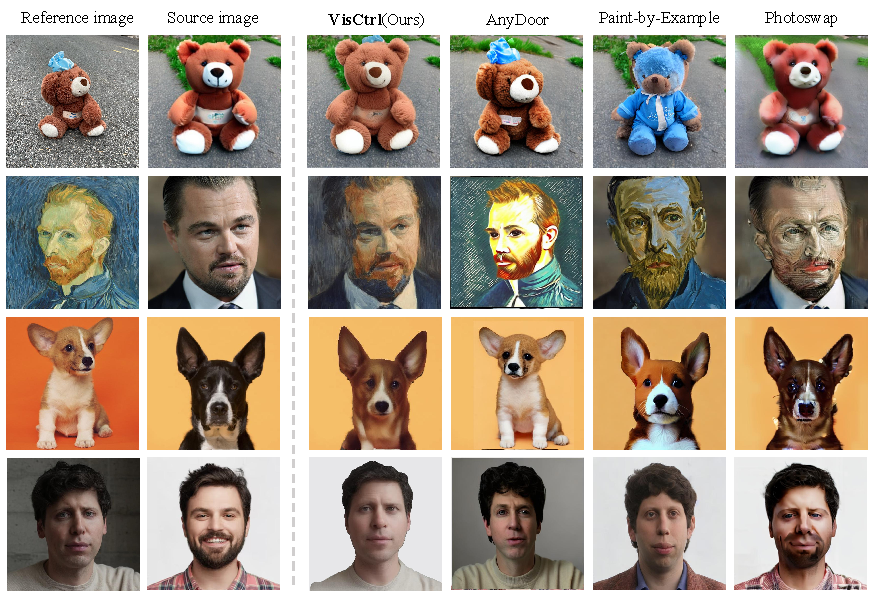
\includegraphics[width=1.000\textwidth]{./figures/VisCtrl/mutil_res.pdf}
  % \vspace{-1mm}
  \caption{不同二维图像编辑方法的效果对比}
  % \vspace{-3mm}
  \label{fig:visctrl_mutil_res}
\end{figure}

VisCtrl能够在将参考主体无缝引入源图像的同时，良好地保留原始主体的关键属性，例如空间布局、几何结构以及姿态等。该方法不仅可以实现相似主体之间的个性化注入，还能够支持不同主体之间的风格迁移。这一能力对于三维数字人的外观编辑具有重要意义——在实际应用中，用户往往需要将特定参考图像中的外观风格（如服饰造型、配饰样式等）迁移到数字人模型上，而VisCtrl的无训练特征注入机制恰好为此提供了高效的解决方案。

\begin{figure}[t]
  \centering
    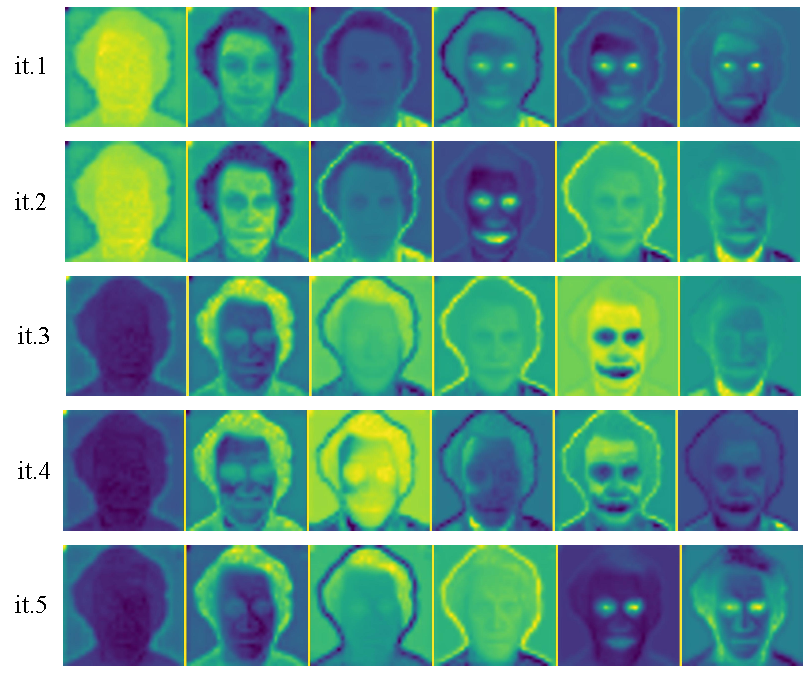
\includegraphics[width=0.800\textwidth]{./figures/VisCtrl/vis_self_attention.pdf}
  % \vspace{-1mm}
  \caption{不同迭代阶段的自注意力图变化}
  % \vspace{-3mm}
  \label{fig:vis_self_attention}
\end{figure}


在图~\ref{fig:visctrl_mutil_res}中，对比分析了本章方法与各基线方法的表现。AnyDoor生成的图像能够较好地呈现参考图像中与主体相关的特征，但会导致源图像结构出现退化。Paint-by-Example的生成质量较高，但无法有效注入主体相关特征，且对源图像的布局结构保留不足。Photoswap在一定程度上同时保留了主体特征与源图像的布局结构，但其生成质量相对较差。相比之下，本章方法显著优于上述基线：在更好地保留源图像布局结构与背景的同时，能够从参考图像中注入更多主体特征，实现了两者之间的有效平衡。在图~\ref{fig:vis_self_attention}中，进一步观察了生成过程中不同迭代阶段自注意力的变化趋势，结果表明编辑后图像的布局信息从初始迭代起就内嵌于自注意力图中。

\subsubsection{三维数字人外观编辑可视化分析}
为进一步验证所提特征注入机制的有效性，在不同迭代次数下分析了不同提示词条件下生成图像的变化及其对应的交叉注意力图。如图~\ref{fig:visctrl_cross_attention}所示，左侧为使用VisCtrl方法将文本条件为$\textprompt_s$的参考图像外观注入到文本条件为$\textprompt_t$的目标图像中的过程。右侧展示了目标图像在迭代过程中的变化，以及其中间潜变量分别与$P_s$和$P_t$计算的交叉注意力图的变化，仅需4次迭代即可获得与9次迭代相当的生成质量。随着迭代推进，参考图像中"joker"的特征逐步变得更加丰富（例如第二次迭代出现的黑眼圈、第三次迭代出现的额头皱纹等）。利用公式~\ref{eq:attention}计算与$\textprompt_t$相关的交叉注意力图，其中输入为目标分支的潜变量（见图~\ref{fig:visctrl_pipeline}下半部分），可以观察到"joker"相关特征持续增强，如图中间行所示。类似地，计算与$\textprompt_s$相关的交叉注意力图，其中输入为参考分支的潜变量（见图~\ref{fig:visctrl_pipeline}上半部分），可以看到"man"相关特征逐渐减弱，如图底部行所示。这种渐进式的特征注入特性使得VisCtrl在应用于三维数字人外观编辑时，能够精确控制外观迁移的程度，避免过度编辑破坏数字人的整体结构。

\begin{figure}[t]
  \centering
    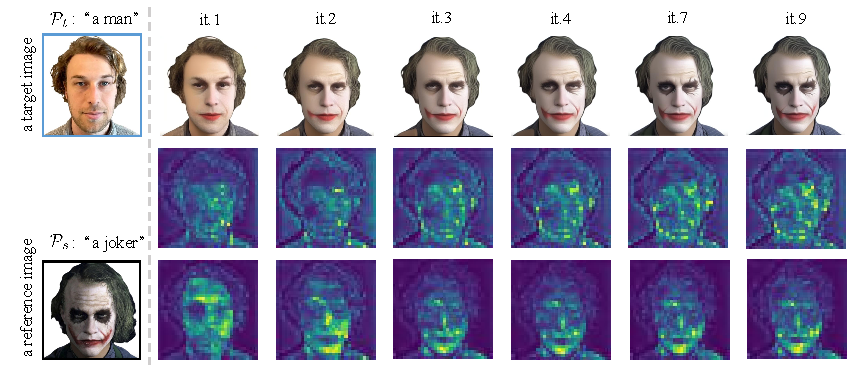
\includegraphics[width=1.000\textwidth]{./figures/VisCtrl/vis_cross_attention.pdf}
  % \vspace{-1mm}
  \caption{不同迭代次数下的交叉注意力图变化}
  % \vspace{-3mm}
  \label{fig:visctrl_cross_attention}
\end{figure}


三维数字人外观编辑的可视化结果如图~\ref{fig:visctrl_3d_baseline}所示，本章方法在三维编辑质量上显著优于现有基线方法。具体而言，Instruct-NeRF2NeRF由于完全依赖文本条件进行编辑，缺乏对目标外观的精细控制能力，导致生成结果在局部结构上出现缺失，同时对背景区域产生不期望的干扰。AnyDoor虽然能够利用参考图像引导编辑方向，但由于缺乏跨视角一致性机制，不同视角间的编辑结果存在明显差异，这种差异在3DGS训练过程中被放大，最终导致渲染结果出现噪声与伪影。而本章方法得益于VisCtrl的迭代式特征注入机制与FGS的多视角一致性保障，能够在多个视角上生成一致的编辑结果，使得3DGS模型能够稳定收敛，从而获得高质量的三维数字人外观编辑效果。


\subsection{消融实验}
\textbf{特征渐进采样对三维数字人外观编辑的作用。} 特征渐进采样是实现三维数字人多视角一致外观编辑的核心策略。在三维数字人的多视角训练数据中，不同视角下的外观变化显著，仅依赖单张参考图像进行编辑时，参考图像所包含的主体信息可能不足，从而在迭代注入过程中导致源图像的部分结构细节被逐步削弱甚至丢失。如图~\ref{fig:visctrl_gfs_fusion}上排所示，图中上排展示了将单张参考图像的特征注入源图像的过程，以及每次迭代中生成图像的变化。在缺乏多视角参考信息时，结构细节逐步丢失，红色圆圈标注的特征会在多层迭代过程中逐渐变弱并最终消失（例如标志"N"的缺失）。一旦这些结构信息在迭代过程中被破坏，后续阶段往往难以将其恢复，因为目标图像分支的表征中已不再包含对应的结构线索。下排展示了使用特征渐进采样策略将多张参考图像的特征注入源图像的过程及其生成图像在各迭代步中的变化，该策略通过渐进式融合多视角信息有效保持了结构完整性。在三维数字人外观编辑场景中，这种结构信息的丢失将直接影响3DGS模型的训练质量。FGS能够有效缓解这一问题：通过从多张参考图像中进行渐进式特征采样与注入，在引入参考特征的同时更好地保留源图像的关键结构细节，从而确保多视角编辑结果的一致性与结构完整性。如图~\ref{fig:visctrl_gfs_fusion}（下排）所示，FGS在实现多参考特征融合的同时，显著提升了结构保真度与细节稳定性。

\begin{figure}[t]
  \centering
    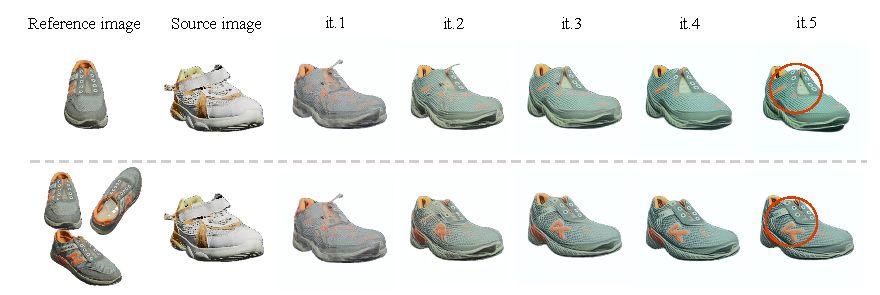
\includegraphics[width=1.000\textwidth]{./figures/VisCtrl/gfs_fusion.pdf}
  % \vspace{-1mm}
  \caption{特征渐进采样策略的消融实验}
  % \vspace{-3mm}
  \label{fig:visctrl_gfs_fusion}
\end{figure}

\textbf{数字人外观身份可控性的消融实验。} 在三维数字人外观编辑中，用户可能需要对外观迁移的程度进行精细控制——例如，有时仅需微调配饰风格，有时则需要进行整体外观的大幅迁移。通过设置起始反演步$T$和起始去噪层$L$，来控制从何时、在网络的哪些层开始启用VisCtrl。不同的$T$与$L$配置会产生不同的编辑效果，如图~\ref{fig:visctrl_diff_step}所示，左边为源图像和参考图像及其对应的文本提示，右上角是改变起始反演步$T$后的编辑效果，随着$T$增大参考图的特征也越来越丰富，但是也会逐渐破坏掉原始图像的结构，意味着反演早期确定形状，反演后期决定纹理；右下角是改变起始去噪层$L$后的编辑效果，此时生成结果在外观上会更接近参考图像，同时在结构层面保持与源图像接近，主体身份迁移程度相对降低。这种灵活的可控性使得VisCtrl在三维数字人外观编辑中能够适应不同粒度的定制需求。

\begin{figure}[!th]
  \centering
    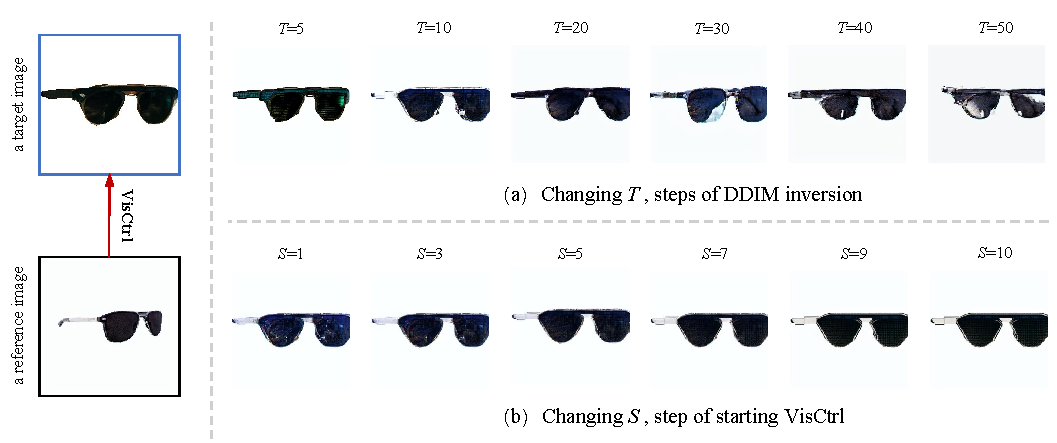
\includegraphics[width=1.000\textwidth]{./figures/VisCtrl/diff_step.pdf}
  % \vspace{-1mm}
  \caption{操控不同去噪步$S$和网络层$L$的编辑结果}
  % \vspace{-3mm}
  \label{fig:visctrl_diff_step}
\end{figure}

% \begin{figure}[!th]
%   \centering
%     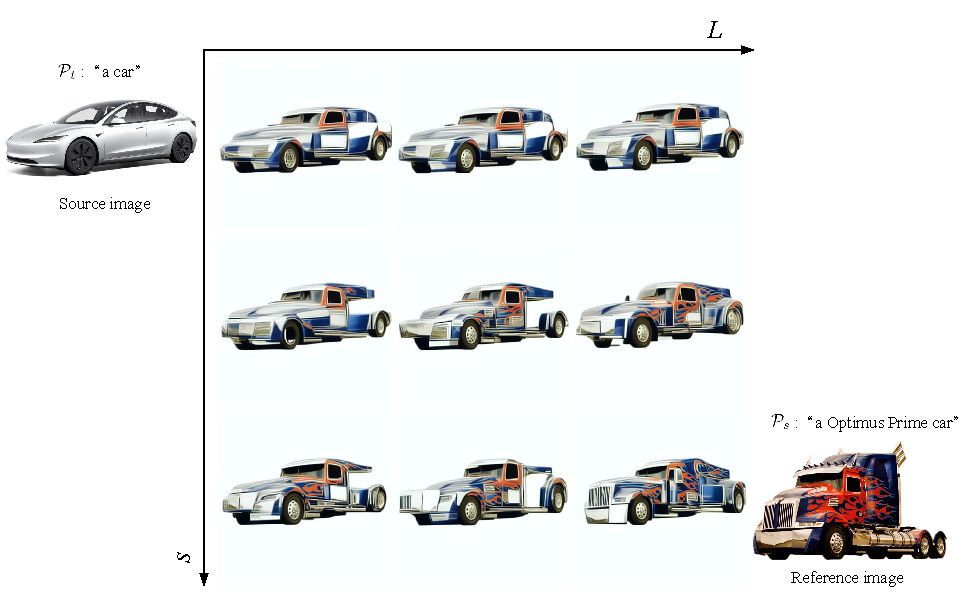
\includegraphics[width=1.000\textwidth]{./figures/VisCtrl/shape_ctrl.pdf}
%   % \vspace{-1mm}
%   \caption{不同注入层与去噪步数组合下的编辑结果}
%   % \vspace{-3mm}
%   \label{fig:visctrl_shape_ctrl}
% \end{figure}

\section{本章小结}
本章提出了视角迭代自注意力控制（VisCtrl），一个面向三维数字人外观个性化编辑的高效框架。VisCtrl无需对模型进行微调，即可利用迭代式自注意力机制在图像之间实现外观特征的精准注入与迁移，仅依赖单张参考图像即可完成数字人外观的快速定制。此外，本章进一步提出面向三维数字人的特征渐进采样策略，通过在多次迭代中平滑融合来自不同视角的外观信息，显著提升编辑结果在跨视角场景下的一致性，从而将所提框架自然拓展至基于3DGS的三维数字人外观编辑任务。本章在示例引导的视觉编辑任务中对该方法进行了验证，覆盖二维图像、视频以及真实三维数字人场景，并在定量与定性评估中均优于现有方法。这一能力为全身舞蹈动作生成提供了风格明确且视觉一致的角色外观基础，使数字人在舞蹈表演中能够兼具个性化外观与高表现力动作，从而在外观生成与舞蹈生成两个维度共同服务于高表现力数字人的整体目标。
